\documentclass[a4paper,12pt]{article}
\usepackage[a4paper,top=1.3cm,bottom=2cm,left=1.5cm,right=1.5cm,marginparwidth=0.75cm]{geometry}
\usepackage{setspace}
\usepackage{cmap}
\usepackage{mathtext}
\usepackage[T2A]{fontenc}
\usepackage[utf8]{inputenc}
\usepackage[english,russian]{babel}
\usepackage{multirow}
\usepackage{graphicx}
\usepackage{wrapfig}
\usepackage{tabularx}
\usepackage{float}
\usepackage{longtable}
\usepackage{hyperref}
\hypersetup{colorlinks=true,urlcolor=blue}
\usepackage[rgb]{xcolor}
\usepackage{amsmath,amsfonts,amssymb,amsthm}
\usepackage{icomma}
% $\mathtoolsset{showonlyrefs=false}$
\usepackage{euscript}
\usepackage{mathrsfs}
\usepackage{float}
\usepackage{amsmath}
\setlength{\parindent}{1cm} % Устанавливает отступ в 1.5 см для всех абзацев


\DeclareMathOperator{\sgn}{\mathop{sgn}}
\newcommand*{\hm}[1]{#1\nobreak\discretionary{}
	{\hbox{$\mathsurround=0pt #1$}}{}}

\title{\textbf{Отчёт о выполненой лабораторной работе \\ \textit{Исследование взаимной диффузии газов (2.2.1)}}}

\author{Каплин Артём Б01-402}
\date{20 апреля 2025}


\begin{document}

\maketitle
	
	\section{Введение}
	
	\textbf{Цель работы:} определение коэффициента диффузии гелия в воздухе.\\
    \\
    \textbf{Оборудование:} форвакуумный насос; баллон с гелием; манометр; источник питания; магазин сопротивления; мультиметр; измерительная установка; компьютер с программой для проведения измерений.
	
	\section{Теоретические сведения }

    \textit{Диффузией}  называют самопроизвольное взаимное проникновение веществ друг в друга происходящее вследствие хаотичного теплового движения молекул. При перемешивании молекул разного сорта говорят о взаимной (или концентрационной) диффузии. В системе, состоящей из двух компонентов a и b (бинарная смесь), плотности потоков частиц в результате взаимной диффузии определяются законом Фика:
        \begin{equation}
            j_a = -D \frac{\partial n_a}{\partial x}, \, j_b = -D \frac{\partial n_b}{\partial x},
        \end{equation}
        где $D$ — \textit{коэффициент взаимной диффузии компонентов}. Знак <<минус>> отражает тот факт, что диффузия идёт в направлении выравнивания концентраций. Равновесие достигается при равномерном распределении вещества по объёму.

        В данной работе исследуется взаимная диффузия гелия и воздуха. Отметим, что давление и температура в системе предполагаются неизменным: $P_0 = (n_{He}+n_{Air})kT = const$, где $n_{He}$  и $n_{Air}$ -- концентрации диффундирующих газов. Поэтому для любых изменений концентраций справедливо $\Delta n_{Air} = -\Delta n_{He}$. Следовательно, достаточно ограничиться описанием диффузии одного из компонентов, например гелия.

        Приведём теоретическую оценку для коэффициента диффузии. В работе концентрация гелия, как правило, мала ($n_{He} \ll n_{Air}$). Кроме того, атомы гелия легче молекул, составляющих воздух ($m_{He} \ll m_{N_2}, m_{O_2}$), значит их средняя тепловая скорость велика по сравнению с остальными частицами. Поэтому перемешивание газов в работе можно приближенно описывать как диффузию примеси лёгких частиц He на практически стационарном фоне воздуха. Коэффициент диффузии в таком приближении равен
        \begin{equation}
            \label{D}
            D = \frac{1}{3} \lambda \langle v \rangle,
        \end{equation}
        где $\lambda = \frac{1}{n\sigma}$ -- длина свободного пробега диффундирующих частиц; $\langle v \rangle = \sqrt{\frac{8kT}{\pi m}}$ -- их средняя тепловая скорость.

        Предполагая, что процесс диффузии будет квазиостационарным, покажем, что разность концентраций будет убывать по экспоненциальному закону
        \begin{equation}
            \label{Delta_n}
            \Delta n = \Delta n_0 e^{-t / \tau},
        \end{equation}
        где $\tau = \frac{VL}{2DS}$ -- характерное время выравнивания концентраций между сосудами, $\Delta n_0$ -- разность концентраций примеси в сосудах в начальный момент
    времени.\\

    \subsection{Метод измерения}

        Рассмотрим подзадачу о диффузии в соединительной трубке. Предположим сперва, что концентрации примеси (гелия) на её торцах поддерживаются постоянными и равными $n_1$ и $n_2$ соответственно. Тогда через некоторое время (оценку этого времени см. ниже формулу (9)) в трубке установится стационарный поток частиц, одинаковый в каждом сечении трубки (в противном случае, если бы поток зависел от $x$, частицы бы накапливались в трубке, и процесс перестал бы быть стационарным). Применяя закон Фика в трубке, получим

        \begin{equation}
            j = -D \frac{\partial n}{\partial x} = \text{const}.
        \end{equation}
        
        Следовательно, распределение концентрации в трубке $n(x)$ — линейная функция:
        
        \begin{equation}
            n(x) = \frac{\Delta n}{L} x,
        \end{equation}
        
        и плотность потока частиц всюду постоянна и равна:
        
        \begin{equation}
            j = -D \frac{\Delta n}{L},
        \end{equation}
        
        где $\Delta n = n_2 - n_1$ — разность концентраций гелия на концах трубки.
        
        Теперь вернёмся к процессу выравнивания концентраций в сосудах. Частицы перетекают из сосуда 2 в сосуд 1 по трубке, и концентрации $n_1(t)$ и $n_2(t)$ меняются во времени. Предположим, что этот процесс происходит достаточно медленно, так что в трубке в любой момент времени успевает установиться практически стационарное течение, описываемое формулами (3), (4). Такое приближение называют \textit{квазистационарным}.
        
        Кроме того, будем считать, что в пределах каждого сосуда частицы распределены равномерно, так что концентрации примеси вблизи трубки и в остальных частях сосуда отличаются мало. Тогда полное число частиц примеси в сосудах равно соответственно $N_1 = n_1 V$ и $N_2 = n_2 V$. Произведение плотности потока (4) на площадь сечения трубки $S$ даёт количество частиц, пересекающих в единицу времени любое поперечное сечение трубки. Поэтому:
        
        \begin{equation}
            \frac{dN_1}{dt} = jS, \quad \frac{dN_2}{dt} = -jS.
        \end{equation}
        
        Вычитая из второго равенства первое и деля результат на объём сосуда $V$, с учётом (6), получим:
        
        \begin{equation}
            \frac{d(\Delta n)}{dt} = -\frac{\Delta n}{\tau},
        \end{equation}
        
        где введено обозначение:
        
        \begin{equation}
            \tau = \frac{1}{D} \cdot \frac{VL}{2S}.
        \end{equation}
        
        Интегрируя (8), получаем, что разность концентраций будет убывать по экспоненциальному закону:
        
        \begin{equation}
            \Delta n = \Delta n_0 e^{-t/\tau},
        \end{equation}
        
        где $\Delta n_0$ — разность концентраций примеси в сосудах в начальный момент времени. \

        \subsection{Экспериментальная установка}
        Схема измерительной части установки приведена на рис.~\ref{fig:setup}. Она соединена с системой откачки и напуска воздуха и гелия. Для откачки используется форвакуумный насос. Конструкции системы откачки и напуска могут быть различны в зависимости от установки (схемы и описания см. на столах); один из вариантов изображён на рис.~\ref{fig:pump}.

        Часть установок компьютеризировано, что позволяет записывать зависимость показаний вольтметра $U(t)$ в реальном времени (на остальных установках фиксация $U(t)$ ведётся вручную с помощью секундомера).
        
        \begin{figure}[h!]
            \centering
            \begin{minipage}[t]{0.45\textwidth}
                \centering
                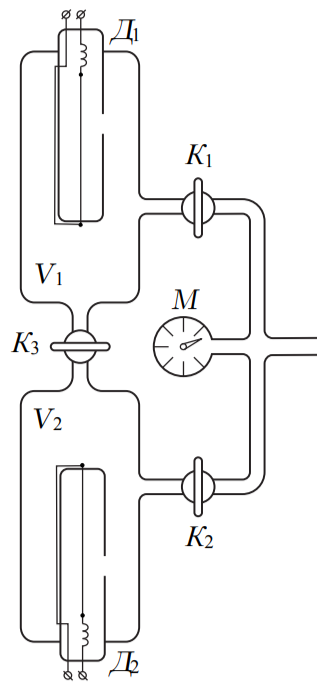
\includegraphics[width=0.6\textwidth]{ust.png}
                \caption{}
                \label{fig:setup}
            \end{minipage}
            \hfill
            \begin{minipage}[t]{0.45\textwidth}
                \centering
                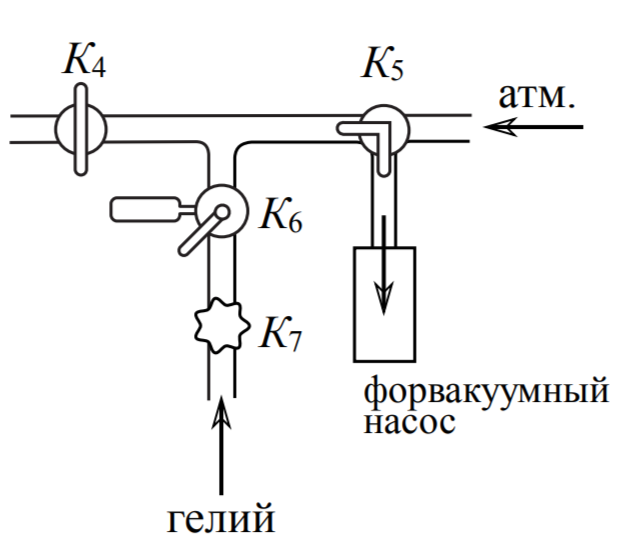
\includegraphics[width=0.9\textwidth]{nasos.png}
                \caption{}
                \label{fig:pump}
            \end{minipage}
        \end{figure}

        
        Измерительная часть установки состоит из двух сосудов $V_1$ и $V_2$, размещённых вертикально. Краны $K_1$ и $K_2$ служат для управления откачкой и подачей воздуха/гелия в сосуды. Диффузия осуществляется через тонкую короткую трубку, соединяющую сосуды, оснащённую краном $K_3$. К соединительным трубкам подключён манометр $M$, измеряющий разность давлений между соединительными трубками и атмосферой и позволяющий измерять давления в разных частях системы (в зависимости от положения кранов).
        
        Выравнивание давлений в сосудах $V_1$ и $V_2$ без изменения состава газов в них может быть осуществлено через обводные трубки посредством кратковременного открытия кранов $K_1$ и $K_2$ (при закрытом $K_3$).
        
        Гелий содержится в баллоне (не изображён на рисунке) под давлением, превышающим атмосферное. Для предотвращения избыточного расхода гелия и его неконтролируемого проникания в установку предусмотрен металлический кран $K_7$, отделяющий её от баллона с гелием. Его открывают только на время непосредственного заполнения установки гелием, остальное время он должен быть закрыт.
        
        Для подачи малых порций гелия предусмотрен двухходовой кран с дозатором (рис.~\ref{fig:doser}). При повороте рычажка $P$ в положение I гелий в небольшом количестве поступает в дозатор (если открыт $K_7$), а при повороте $P$ в положение II порция из дозатора поступает в установку.
        
         \begin{figure}[h!]
            \centering
            \begin{minipage}[t]{0.45\textwidth}
                \centering
                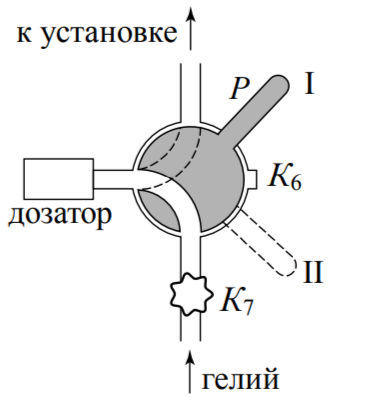
\includegraphics[width=0.9\textwidth]{dozator.png}
                \caption{}
                \label{fig:doser}
            \end{minipage}
            \hfill
            \begin{minipage}[t]{0.45\textwidth}
                \centering
                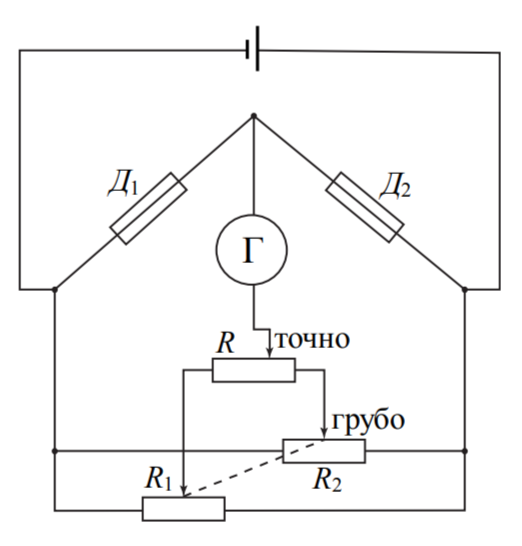
\includegraphics[width=0.9\textwidth]{cep.png}
                \caption{}
                \label{fig:bridge}
            \end{minipage}
        \end{figure}

        
        Датчики теплопроводности $\text{Д}_1$ и $\text{Д}_2$, расположенные в сосудах $V_1$ и $V_2$ соответственно, включены в мостовую электрическую схему согласно рис.~\ref{fig:bridge}. В одну из диагоналей моста включён высокочувствительный вольтметр (гальванометр) $G$, к другой подключается источник небольшого постоянного напряжения. Сопротивления проволок датчиков составляют одно из плеч моста. Второе плечо составляют переменные сопротивления $R_1$, $R_2$ и $R$, служащие для установки показаний вольтметра $G$ на нуль (балансировка моста).
        
        Сопротивления $R_1$ и $R_2$ спарены (их подвижные контакты находятся на общей оси) и изменяются одновременно при повороте ручки грубой регулировки. Точная балансировка выполняется потенциометром $R$. Балансировку необходимо проводить перед каждым экспериментом заново: при этом установка заполняется чистым газом (воздухом без гелия) при давлении, близком «рабочему» (при котором затем будут проводиться измерения).

        \section{Приборы и данные}

        \begin{itemize}
            \item Цифровой мульиметр Вольтметр универсальный B7-78, погрешность измерения постоянного напряжения 0,0035\% + 0,0005\% диапазона мВ;
            \item Форвакуумный насос Адвавак 2, скорость откачки 2 м$^3$/час;
            \item Источник постоянного напряжения GW Instek GPS-2303, погрешность 0,5\% + 10 мВ;
            \item Вакуумметр образцовый ГОСТ 6521-60, класс точности 0,4.
        \end{itemize}
        \newpage
        \section{Ход работы}

        \begin{enumerate}
    \item \textbf{Ознакомление с установкой:}
    \begin{itemize}
        \item Изучили схему подачи воздуха и гелия, а также схему откачки установки согласно дополнительному описанию, расположенному на рабочем столе.
        \item Ознакомились с особенностями измерительных приборов: манометра и вольтметра. Определили цену деления шкалы манометра в торрах: 1 деление = 7,45 торр.
      
    \end{itemize}

    \item \textbf{Подготовка установки к работе:}
    \begin{itemize}
        \item Подсоединили установку к форвакуумному насосу согласно схеме откачки и провели откачку до давления порядка $0{,}1$ торр.
        \item После откачки выключили насос в два этапа:
        \begin{enumerate}
            \item Сначала выключили питание насоса.
            \item Затем соединили насос с атмосферой, чтобы избежать попадания масла в установку.
        \end{enumerate}
    \end{itemize}

    \item \textbf{Балансировка измерительного моста:}
    \begin{itemize}
        \item Напустили в установку воздух до суммарного давления $P_\Sigma \approx 50$ торр.
        \item При избыточном давлении — произвели частичную откачку до нужного значения.
        \item Изолировали рабочие объемы, закрыв краны К1 и К2, оставив открытым кран К3.
        \item Сбалансировали измерительный мост:
        \begin{itemize}
            \item Использовали ручки «грубой» и «точной» настройки.
            \item Добились того, чтобы показания вольтметра флуктуировали около нулевого значения.
        \end{itemize}
    \end{itemize}

    \item \textbf{Приготовление рабочих газовых смесей:}
    \begin{itemize}
        \item Повторно откачали всю установку до давления порядка $0{,}1$ торр.
        \item Изолировали объем $V_2$, закрыв краны К2 и К3 — важно, чтобы в этот сосуд не попал гелий.
        \item Напустили в установку гелий до давления $P_{\text{He}} = 0{,}2 \cdot P_\Sigma$.
        \item При превышении давления — удалили избыточное количество гелия форвакуумным насосом.
        \item Изолировали объем $V_1$ с помощью крана К1.
        \item Перекрыли кран подачи гелия К7.
        \item Произвели откачку гелия из всех патрубков установки, затем остановили откачку.
        \item Присоединили объем $V_2$ к установке (открыли кран К2) и напустили воздух до давления, превышающего рабочее (примерно $1{,}7 \cdot P_\Sigma$).
        \item Уравняли давления между $V_1$ и $V_2$:
        \begin{itemize}
            \item Открыли краны К1 и К2 при закрытых К3 и К4.
            \item Подождали 30–60 секунд, чтобы температуры в сосудах сравнялись.
            \item Не допускали слишком долгой выдержки, чтобы избежать диффузии гелия в обратном направлении.
        \end{itemize}
        \item Зафиксировали точное значение установившегося давления $P_\Sigma$.
        \item Изолировали объёмы $V_1$ и $V_2$, закрыв краны К1 и К2.
    \end{itemize}

    \item \textbf{Проведение измерений:}
    \begin{itemize}
        \item Подготовили компьютерную программу для записи зависимости напряжения $U(t)$ от времени.
        \item Открыли кран К3 и начали процесс диффузии.
        \item Продолжали измерения до тех пор, пока напряжение не уменьшилось минимум на 40-50\%.
    \end{itemize}

    \item \textbf{Повторение эксперимента:}
    \begin{itemize}
        \item Повторили шаги по приготовлению смеси и измерению при других значениях $P_\Sigma$.
        \item Провели 6 серий измерений в диапазоне $50 \div 220$ торр.
    \end{itemize}
    \end{enumerate}

    \section{Обработка результатов и измерений}

    \begin{enumerate}
        \item По полученным данным построим графики зависимости напряжения от времени $U(t)$, а также эту же зависимость в логарифмическом масштабе по оси оридинат.

        \begin{figure}[h!]
            \centering{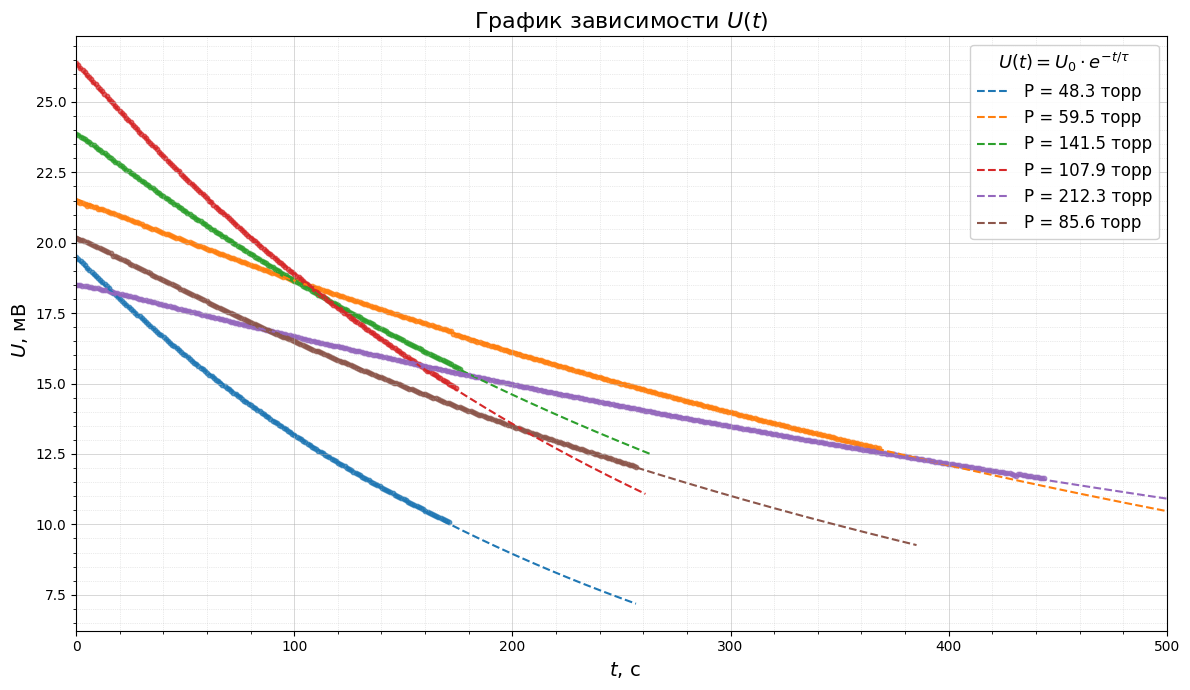
\includegraphics[width=1\textwidth]{gr1png.png}}
            \caption[]{\label{} Экспоненциальная зависимость напряжения от времени}
        \end{figure}
        
        \begin{figure}[h!]
            \centering{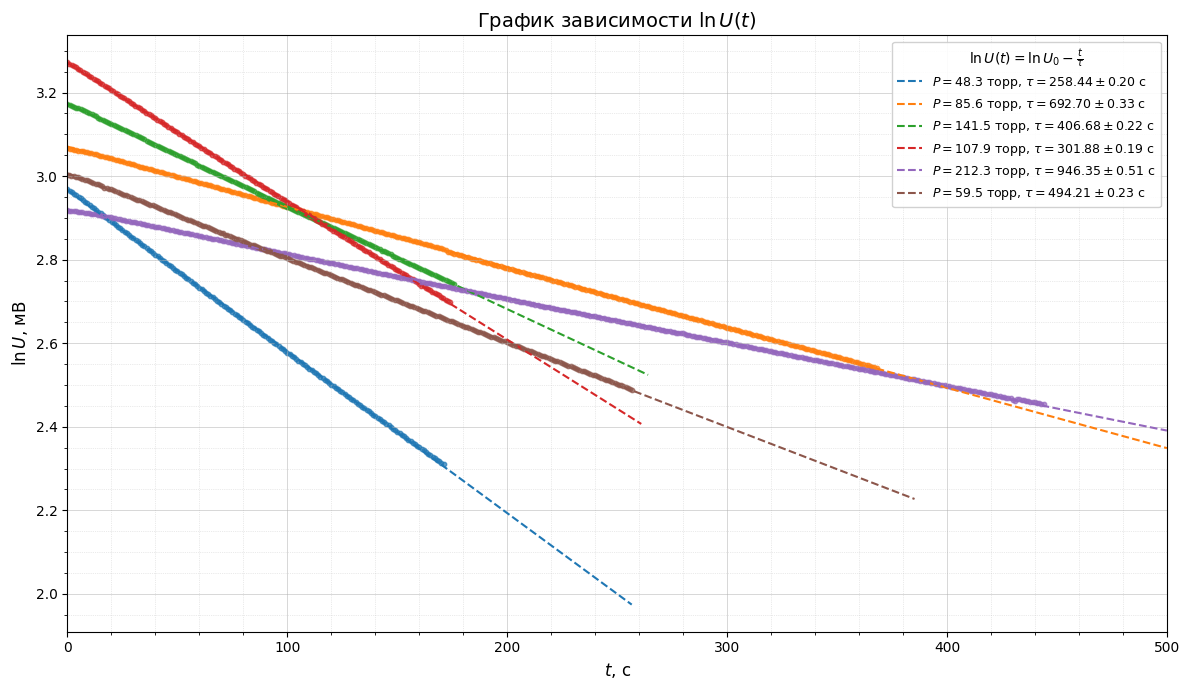
\includegraphics[width=1\textwidth]{gr2.png}}
            \caption[]{\label{}Зависимость логарифма напряжения от времени}
        \end{figure}

        \item По угловым коэффициентам и известным геометрическим параметрам установки рассчитали коэффициенты взаимной диффузии при выбранных рабочих давлениях (формулы (9) и (10) ). Полученные данные в таблице.

        \begin{align*}
            \sigma_D &= D \sqrt{\left( \frac{\sigma_{L/S}}{L/S} \right)^2 + \left( \frac{\sigma_V}{V} \right)^2 + \left( D \frac{\sigma_k}{k} \right)^2}\\
        \end{align*}

        \begin{table}[h!]
    \centering
    \begin{tabular}{|c|c|c|c|c|c|c|}
        \hline
        $P,  \ \text{дел}$ & $P, \  \text{торр}$ & $\tau,  \ \text{с}$ & $D, \frac{\text{см}^2}{\text{с}}$ & $\sigma_D, \frac{\text{см}^2}{\text{с}}$ & $\varepsilon_D, \%$ \\
        \hline
        $6.5 \pm 0.4$   & $48.4 \pm 3.0$  & $258.44 \pm 0.20$ & 7.31 & 0.19 & 2.63 \\ \hline
        $8.0 \pm 0.4$   & $59.5 \pm 3.0$  & $301.88 \pm 0.19$ & 6.26 & 0.16 & 2.63 \\ \hline
        $11.5 \pm 0.4$  & $85.6 \pm 3.0$  & $406.68 \pm 0.22$ & 4.65 & 0.12 & 2.63 \\ \hline
        $14.5 \pm 0.4$  & $108.0 \pm 3.0$ & $494.21 \pm 0.23$ & 3.82 & 0.10 & 2.63 \\ \hline
        $19.0 \pm 0.4$  & $141.5 \pm 3.0$ & $692.70 \pm 0.33$ & 2.73 & 0.07 & 2.63 \\ \hline
        $28.5 \pm 0.4$  & $212.3 \pm 3.0$ & $946.35 \pm 0.51$ & 2.00 & 0.05 & 2.63 \\
        \hline
    \end{tabular}
    \caption{Зависимость времени релаксации $\tau$ и диаметра пятна $D$ от давления $P$}
\end{table}

    \item По получненным коэффициентам диффузии построим по методу $\chi^2$ зависимость $D(\frac{1}{P})$. 

    \begin{figure}[h!]
            \centering{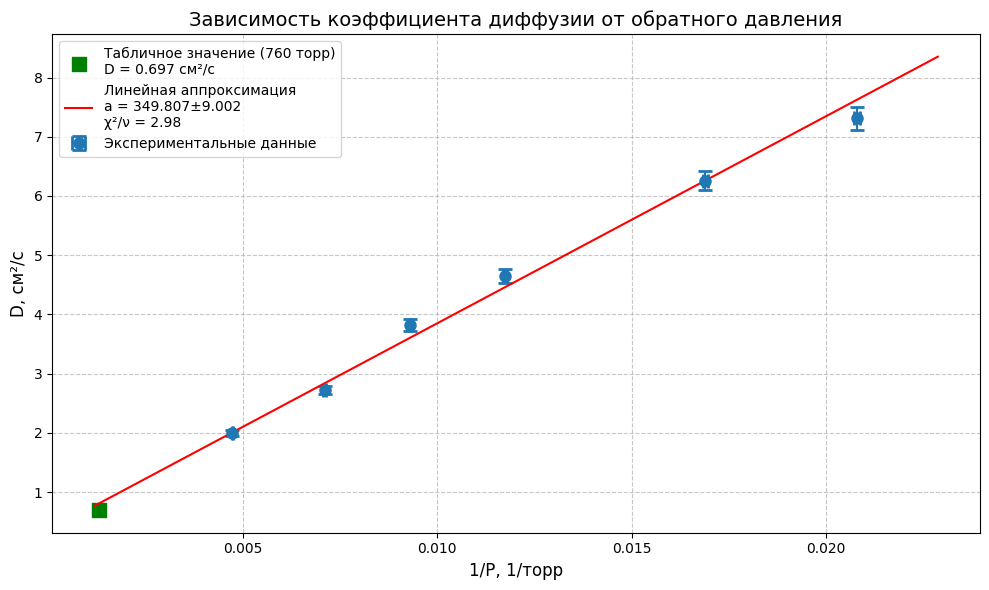
\includegraphics[width=1\textwidth]{gr3.png}}
            \caption[]{\label{} Зависимость коэффициента диффузии от обратного давления $D(\frac{1}{P})$}
        \end{figure}
        
    % \newpage


\item Исходя из известных параметров, рассчитаем концентрацию молекул воздуха $n_0^1$ при давлении $P_1$, а также длину свободного пробега $\lambda_{He}$ и эффективное сечение столкновений $\sigma_{He_{\text{возд}}}$:

\begin{equation*}
    n_0^1 = \frac{P_1}{kT_0} = \frac{48{,}4 \cdot 133{,}322}{1{,}38 \cdot 10^{-23} \cdot 298} \approx 1{,}57 \cdot 10^{24}~\text{м}^{-3}
\end{equation*}
\begin{equation*}
    \sigma_{n_0^1} = n_0^1 \cdot \frac{\sigma_{P_1}}{P_1} = 1{,}57 \cdot 10^{24} \cdot \frac{3}{48{,}4} = 9{,}8 \cdot 10^{22}~\text{м}^{-3}
\end{equation*}

Средняя скорость гелия при температуре $T = 298$~K:

\begin{equation*}
    \bar{v} = \sqrt{\frac{8RT}{\pi \mu}} = \sqrt{\frac{8 \cdot 8{,}31 \cdot 298}{3{,}1415 \cdot 4 \cdot 10^{-3}}} = 1255{,}6~\frac{\text{м}}{\text{с}}
\end{equation*}

Длина свободного пробега:

\begin{equation*}
    \lambda_1 = \frac{3D}{\bar{v}} = \frac{3 \cdot 7{,}31 \cdot 10^{-4}}{1255{,}6} \approx 1747{,}3~\text{нм}
\end{equation*}
\begin{equation*}
    \sigma_{\lambda_1} = \lambda_1 \cdot \varepsilon_{D_1} = 45{,}9~\text{нм}
\end{equation*}

Соответствующее эффективное сечение:

\begin{equation*}
    \sigma_{He}^1 = \frac{1}{n_0^1 \lambda_1} = \frac{1}{1{,}57 \cdot 10^{24} \cdot 1747{,}3 \cdot 10^{-9}} \approx 3{,}65 \cdot 10^{-19}~\text{м}^2
\end{equation*}
\begin{equation*}
    \sigma_{\sigma_{He}^1} = \sigma_{He}^1 \cdot \sqrt{\left(\frac{\sigma_{n_0^1}}{n_0^1}\right)^2 + \left(\frac{\sigma_{\lambda_1}}{\lambda_1}\right)^2} = 2{,}48 \cdot 10^{-20}~\text{м}^2
\end{equation*}

\end{enumerate}

\begin{table}[H]
    \centering
    \begin{tabular}{|c|c|c|c|c|c|c|c|}
        \hline
        $P,\ \text{торр}$ & $n_0,\ 10^{24}$~м$^{-3}$ & $\sigma_{n_0},\ 10^{24}$~м$^{-3}$ & $\lambda$, нм & $\sigma_\lambda$, нм & $\sigma_{He},\ 10^{-19}$~м$^2$ & $\sigma_{\sigma_{He}},\ 10^{-19}$~м$^2$ & $\varepsilon_{\sigma_{He}},\ \%$ \\
        \hline
        48.4 $\pm$ 3.0 & 1.57 & 0.10 & 1747.3 & 45.9 & 3.65 & 0.25 & 6.8 \\ \hline
        59.5 $\pm$ 3.0 & 1.93 & 0.10 & 1495.9 & 39.3 & 3.47 & 0.20 & 5.7 \\ \hline
        85.6 $\pm$ 3.0 & 2.78 & 0.10 & 1110.4 & 29.2 & 3.24 & 0.14 & 4.4 \\ \hline
        108.0 $\pm$ 3.0 & 3.50 & 0.10 & 913.7  & 24.0 & 3.13 & 0.12 & 3.8 \\ \hline
        141.5 $\pm$ 3.0 & 4.59 & 0.10 & 651.9  & 17.1 & 3.34 & 0.11 & 3.4 \\ \hline
        212.3 $\pm$ 3.0 & 6.88 & 0.10 & 477.2  & 12.5 & 3.04 & 0.09 & 3.0 \\ \hline
        756.0 $\pm$ 3.0 & 24.51 & 0.10 & 195.8  & 18.0 & 2.08 & 0.19 & 9.2 \\ \hline
        760.0 $\pm$ 3.0 & 24.64 & 0.10 & 195.2  & 18.0 & 2.08 & 0.19 & 9.2 \\
        \hline
    \end{tabular}
    \caption{Результаты вычислений для различных давлений: концентрация $n_0$, длина пробега $\lambda$ и сечение $\sigma_{He}$.}
\end{table}

Для сравнения воспользуемся табличным значением коэффициента диффузии $D_{\text{табл}} = 0{,}697~\frac{\text{см}^2}{\text{с}}$:

\begin{equation*}
    \lambda_{\text{табл}} = 166{,}5~\text{нм}, \quad \sigma_{\text{табл}} = \frac{1}{n_0^{760} \cdot \lambda_{\text{табл}}} = 2{,}44 \cdot 10^{-19}~\text{м}^2
\end{equation*}

\section{Обсуждение результатов}

\begin{enumerate}
    \item Графики подтверждают выполнение закона диффузии, описываемого формулой (10).
    \item Коэффициент диффузии обратно пропорционален давлению, что следует из графика зависимости $D(P^{-1})$.
    \item Сравнение значения $D$ при $P=760$~торр с табличным:

    \begin{table}[H]
        \centering
        \begin{tabular}{|c|c|c|}
            \hline
            Величина & Эксп. зн. & Табл. зн. \\
            \hline
            $D,\ \frac{\text{см}^2}{\text{с}}$ & 0{,}818 & 0{,}697 \\ \hline
            $\sigma_D,\ \frac{\text{см}^2}{\text{с}}$ & 0{,}075 & 0{,}120 \\ \hline
            $\varepsilon_D,\ \%$ & 9{,}2 & 17{,}2 \\
            \hline
        \end{tabular}
        \caption{Сравнение экспериментального и табличного значений коэффициента диффузии}
    \end{table}

\end{enumerate}

\section{Выводы}

Были выполнены измерения зависимости напряжения от времени при различных давлениях. Построены графики $U(t)$ и $\ln U(t)$, по которым определены коэффициенты диффузии. Получена зависимость $D(P^{-1})$, по которой проведена экстраполяция на атмосферное давление. Также вычислены длина свободного пробега и сечение столкновений при каждом давлении, с последующим сравнением с табличными значениями.

\end{document}
